\documentclass[UTF8,a4paper,12pt]{ctexbook} 

\usepackage{graphicx}%学习插入图
\usepackage{verbatim}%学习注释多行
\usepackage{booktabs}%表格
\usepackage{geometry}%图片
\usepackage{amsmath}
\usepackage{amssymb}
\usepackage{listings}%代码
\usepackage{xcolor}  %颜色
\usepackage{enumitem}%列表格式
\setenumerate[1]{itemsep=0pt,partopsep=0pt,parsep=\parskip,topsep=5pt}
\setitemize[1]{itemsep=0pt,partopsep=0pt,parsep=\parskip,topsep=5pt}
\setdescription{itemsep=0pt,partopsep=0pt,parsep=\parskip,topsep=5pt}
\usepackage{tcolorbox}
\usepackage{algorithm}  %format of the algorithm
\usepackage{algorithmic}%format of the algorithm
\usepackage{multirow}   %multirow for format of table
\usepackage{tabularx} 	%表格排版格式控制
\usepackage{longtable}
\usepackage{array}	%表格排版格式控制
\usepackage{hyperref} %超链接 \url{URL}
\usepackage{tikz}
\usepackage{dirtree}


\usetikzlibrary{intersections,
	positioning,
	petri,
	backgrounds,
	fit,
	decorations.pathmorphing,
	arrows,
	arrows.meta,
	bending,
	calc,
	intersections,
	through,
	backgrounds,
	shapes.geometric,
	quotes,
	matrix,
	trees,
	shapes.symbols,
	graphs,
	math,
	patterns,
	external}
\CTEXsetup[format+={\flushleft}]{section}

%%%% 设置图片目录
\graphicspath{{figure/}}

%%%% 段落首行缩进两个字 %%%%
\makeatletter
\let\@afterindentfalse\@afterindenttrue
\@afterindenttrue
\makeatother
\setlength{\parindent}{2em}  %中文缩进两个汉字位

%%%% 下面的命令重定义页面边距,使其符合中文刊物习惯 %%%%
\addtolength{\topmargin}{-54pt}
\setlength{\oddsidemargin}{0.63cm}  % 3.17cm - 1 inch
\setlength{\evensidemargin}{\oddsidemargin}
\setlength{\textwidth}{14.66cm}
\setlength{\textheight}{24.00cm}    % 24.62

%%%% 下面的命令设置行间距与段落间距 %%%%
\linespread{1.4}
\setlength{\parskip}{0.5\baselineskip}
\geometry{left=1.6cm,right=1.8cm,top=2cm,bottom=1.7cm} %设置文章宽度
\pagestyle{plain} 		  %设置页面布局

%代码效果定义
\definecolor{mygreen}{rgb}{0,0.6,0}
\definecolor{mygray}{rgb}{0.5,0.5,0.5}
\definecolor{mymauve}{rgb}{0.58,0,0.82}
\lstset{ %
	backgroundcolor=\color{white},   % choose the background color
	basicstyle=\footnotesize\ttfamily,      % size of fonts used for the code
	%stringstyle=\color{codepurple},
	%basicstyle=\footnotesize,
	%breakatwhitespace=false,         
	%breaklines=true,                 
	%captionpos=b,                    
	%keepspaces=true,                 
	%numbers=left,                    
	%numbersep=5pt,                  
	%showspaces=false,                
	%showstringspaces=false,
	%showtabs=false,        
	columns=fullflexible,
	breaklines=true,                 % automatic line breaking only at whitespace
	captionpos=b,                    % sets the caption-position to bottom
	tabsize=4,
	commentstyle=\color{mygreen},    % comment style
	escapeinside={\%*}{*)},          % if you want to add LaTeX within your code
	keywordstyle=\color{blue},       % keyword style
	stringstyle=\color{mymauve}\ttfamily,     % string literal style
	frame=L,
	xleftmargin = .079\textwidth,
	rulesepcolor=\color{red!20!green!20!blue!20},
	% identifierstyle=\color{red},
	language=c++,
}
 \author{\kaishu 郑华}
 \title{\heiti Unreal4 笔记}
 
\begin{document}          %正文排版开始
 	\maketitle
 	\tableofcontents


\chapter{GamePlay}
	\section{基础世界观}
		\begin{figure}[H]
			\centering
			\includegraphics[width=\linewidth]{Base}
			\caption{Gameplay Framwork}
		\end{figure}
		
		\begin{itemize}
			\item Game Instance: 从游戏开始到游戏结束,可保存跨场景数据等。
			\item Game Mode: 储存游戏中不经常被修改的数据
			\item Pawn Class:人物、AI 载体实体
			\item HUD Class:二维显示信息
			\item Player Controller Class; 代表玩家的控制:包括输入操作、AI控制等
			\item Player State Class: 玩家的状态信息
			\item Game State Class: 任务状态等
		\end{itemize}
		
	\section{基础元素与组件}
		\subsection{UObject}
			UObject类提供了以下功能:
			\begin{itemize}
				\item 垃圾收集
				\item 引用自动更新
				\item 反射
				\item 序列化
				\item 自动检测 默认变量的更改
				\item 自动变量初始化
				\item 和虚幻引擎编辑器的自动交互
				\item 运行时类型识别
				\item 网络复制
			\end{itemize}
		
		\subsection{Actor}
			Actor类在场景中拥有一个位置坐标和旋转量。
			
			Actor类拥有这样的能力:\textbf{它能够被挂载组件} 。
			
			
		\subsection{Pawn}
			现Pawn类提供了\textit{被“操作”的 特性}。
			
			它能够被一个Controller操纵。这个Controller可以是玩家,当然 也可以是AI(人工智能)。这就像是一个棋手,操作着这个棋子。
			
			这就是Pawn类,一个被操纵的兵或卒,一个一旦脱离棋手就无法 自主行动的、悲哀的肉体。
			
		\subsection{Controller}
			既然是灵魂,那么肉体就不唯一,因此灵魂(Controller) 可以通过 Possess/UnPossess来控制一个肉体,或者从一个肉体上离开。
		
		\subsection{Character}
			Character类代表一个角色,它继承自Pawn类。
			
			Character类提供了一个特殊的组件,Character Movement。这个组 件提供了一个基础的、基于胶囊体的角色移动功能。包括移动和跳跃, 以及如果你需要,还能扩展出更多,例如蹲伏和爬行。


	\section{控制}
		
	
	
	\section{迭代}
		
	
	
	
	\section{命名规则}
		常用的前缀如下:
		\begin{itemize}
			\item F 纯C++类
			\item U 继承自UObject,但不继承自Actor
			\item A 继承自Actor
			\item S Slate控件相关类
			\item H HitResult相关类
		\end{itemize}
		
		
	\section{对象}
		
		\subsection{生成}
			在标准C++中,一个类产生一个对象,被称为“实例化”。实例化对 象的方法是通过new关键字。 而在虚幻引擎中,这一个问题变得略微复杂。对于某些类型,我们 不得不通过调用某些函数来产生出对象。具体而言:
			
			\begin{itemize}
				\item 如果你的类是一个\textbf{纯C++类}型(F开头),你可以通过\textbf{new}来产生对 象。
				\item 如果你的类\textbf{继承自UObject}但不继承自Actor,你需要通过 \textbf{NewObject函数}来产生出对象。 \verb|NewObject<T>()|
				\item 如果你的类\textbf{继承自AActor},你需要通过\textbf{SpawnActor函数}来产生出对 象。\verb|GetWorld()-> SpawnActor<AYourActorClass>()|
				\item 如果你需要产生出一个\textbf{Slate类},需要使用\textbf{SNew函数}。
			\end{itemize}
		
		\subsection{获取}:
		
			1· 通过new 获取引用或者指针。
			
			2·间接的通过遍历对象获取。
			
			\begin{lstlisting}
	for(TActorIterator <AActor> Iterator(GetWorld()); Iterator; ++Iterator) 
	{ ...//do something }			
			\end{lstlisting}
		
		\subsection{销毁}
			\begin{itemize}
				\item 纯C++ 类:符合C++ 基本语法
				\item UObject类:UObject采用自动垃圾回收机制。当一个\textbf{类的成员} 变量包含\textit{指向UObject的对象},\textit{同时又带有UPROPERTY宏定义},那么 这个成员变量将会触发引用计数机制。 垃圾回收器会定期从根节点Root开始检查,当一个UObject没有被 别的任何UObject引用,就会被垃圾回收。你可以通过AddToRoot函数来 让一个UObject一直不被回收。
				\item Actor 类:可以通过\textbf{调用Destory函数}来请求销毁,这样的销毁意 味着将当前Actor从所属的世界中“摧毁”。但是对象对应\textit{内存的回收依然 是由系统决定}。
			\end{itemize}
		
	
	\section{subsystem}
		Subsystems 是一套可以定义、自动实例化和释放的类的框架。 可以理解为后台管理程序,或者游戏运行支持系统。
		
		\subsection{概述}
			\paragraph{更易管理的生命周期}
				引擎只支持一个 GameInstance ,运行周期是整个引擎的生命周期
				
				自定义 ManagerActor,生命周期一般为当前 level 的生命周期
				
				Subsystems 的生命周期可以依存于Engine,Editor,World,LocalPlayer
				
			\paragraph{更简单易生成}
				GameInstance 或者自定义 ManagerActor,需要手动维控制创建、释放
				
				Subsystems 自动创建、释放,提供 Initialize()、Deinitialize(),并且可重载
			
			\paragraph{模块化、代码更易读}
					
			
		\subsection{类关系}
			\begin{figure}[H]
				\centering
				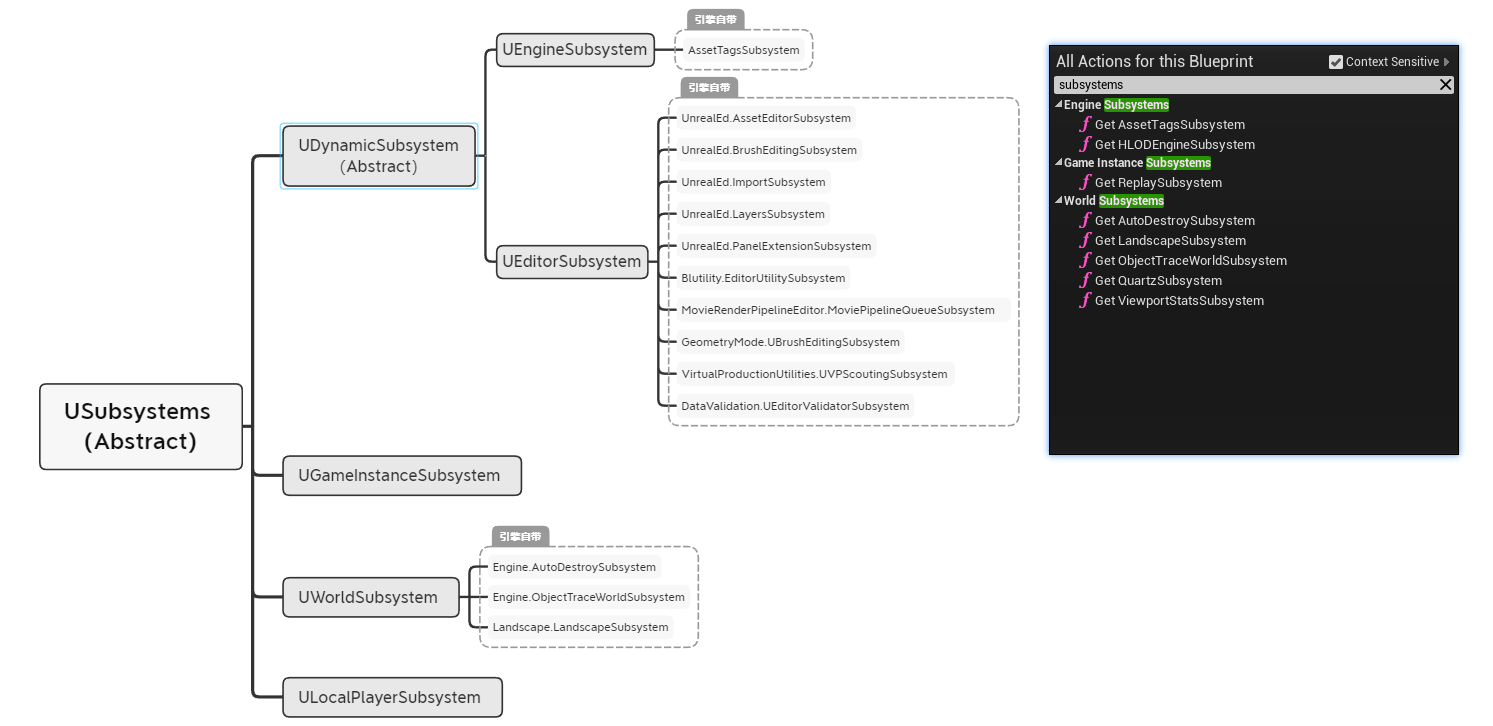
\includegraphics[width=\linewidth]{subsystem}
				\caption{子系统类型及类图}
			\end{figure}
		
		\subsection{生命周期}
			如上:主要描述各种subsystem 的启动时机与销毁时机。
			\begin{itemize}
				\item UDynamicSubsystem
					\begin{itemize}
						\item UEngineSubsystem:\textit{从进程启动开始创建,进程退出时销毁。}
						\item UEditorSubsystem:\textit{从编辑器启动开始创建,到编辑器退出时销毁。}
					\end{itemize}
				\item UGameInstanceSubsystem:\textit{从游戏的启动开始创建,游戏退出时销毁}。这里的一场游戏指的是Runtime或PIE模式的运行的都算,一场游戏里可能会创建多个World切换。
				\item UWorldSubsystem:其生命周期,跟GameMode是一起的。(EWorldType:Game,Editor,PIE,EditorPreview,GamePreview等 )
				\item ULocalPlayerSubsystem:LocalPlayer虽然往往跟PlayerController一起访问,但是其生命周期其实是跟UGameInstance一起的(默认一开始的时候就创建好一定数量的本地玩家),或者更准确的说是跟LocalPlayer的具体数量挂钩(当然你也可以运行时动态调用AddLocalPlayer)。
			\end{itemize}
		
		\subsection{创建示例C++}
			示例代码:
			
			\begin{lstlisting}
	// UMyEngineSubsystem 获取 
	UMyEngineSubsystem* MyEngineSubsystem = GEngine->GetEngineSubsystem<UMyEngineSubsystem>();
	
	// UMyEditorSubsystem 获取
	UMyEditorSubsystem* MyEditorSubsystem = GEditor->GetEditorSubsystem<UMyEditorSubsystem>();
	
	// UMyGameInstanceSubsystem 获取
	//UGameInstance* GameInstance = GetWorld()->GetGameInstance();
	UGameInstance* GameInstance = UGameplayStatics::GetGameInstance();
	UMyGameInstanceSubsystem* MyGameInstanceSubsystem = GameInstance->GetSubsystem<UMyGameInstanceSubsystem>();
	
	// UMyWorldSubsystem 获取
	UMyWorldSubsystem* MyWorldSubsystem = GetWorld()->GetSubsystem<UMyWorldSubsystem>();
	
	// UMyLocalPlayerSubsystem 获取
	ULocalPlayer* LocalPlayer = UGameplayStatics::GetPlayerController()->GetLocalPlayer();
	UMyLocalPlayerSubsystem* MyLocalPlayerSubsystem = LocalPlayer->GetSubsystem<UMyLocalPlayerSubsystem>();		
			\end{lstlisting}
			

\chapter{蓝图}
	\section{基本概念}
	
		蓝图类,类似于prefab,定义一种\textbf{基于事件}的预工作流。
		
		\subsection{分类}
			
			\begin{itemize}
				\item 类蓝图 Blueprint Class:是一种允许内容创建者轻松地基于现有游戏性类添加功能的资源。
				\item 纯数据蓝图 Data-Only Blueprint:是指仅包含\underline{代码(以节点图表的形式)}、\textbf{变量}及\textbf{从其父类继承的组件}的\textit{类蓝图}。
				\item 关卡蓝图 Level Blueprint:用作关卡范围的\textbf{全局事件}图。
			\end{itemize}
		
		\subsection{蓝图接口}
			蓝图接口(Blueprint Interface) 是一个或多个函数的集合 - 只有名称,没有实施-可以添加到其他蓝图中。
		
		\subsection{蓝图宏库}
			蓝图宏库(Blueprint Macro Library) 是一个容器,它包含一组 宏 或自包含的图表,这些图表可以 作为节点放置在其他蓝图中。它们可以节省时间,因为它们可以存储常用的节点序列, 包括执行和数据传输所需的输入和输出。
		
		\subsection{蓝图工具}
			\textbf{蓝图编辑器(Blueprint Editor) 中}的 \textbf{组件(Components) 窗口}允许您\underline{将组件添加到蓝图}。这提供了以下方法: 通过胶囊组件(CapsuleComponent)、盒体组件(BoxComponent)或球体组件(SphereComponent)添加碰撞几何体, 以静态网格体组件(StaticMeshComponent)或金属网格体组件(SkeletalMeshComponent)形式添加渲染几何体, 使用移动组件(MovementComponent)控制移动。还可以将组件(Components)列表中添加的组件 指定给实例变量,以便您在此蓝图或其他蓝图的图表中访问它们。
		
		
		\subsection{核心组件}
			\begin{itemize}
				\item 构造函数 
				\item 事件图表:事件驱动
				\item 函数
				\item 变量
			\end{itemize}
			
	\section{使用规则}
		基于事件。
		
		控制流、数据流。
		
		
	\section{调用C++}
		如何让蓝图能够调用我的 C++类中的函数呢?
		
		\begin{itemize}
			\item \verb|UPROPERTY宏|:注册一个变量到蓝图中\verb|UPROPERTY(BlueprintReadWrite,VisibleAnywhere,Category="Object")|
			\item \verb|UFUNCTION宏|:注册函数到蓝图中 \verb|UFUNCTION(BlueprintCallable,Category="Test")|
		\end{itemize}
	
		
\chapter{事件}




	
\chapter{委托}
	\section{概述}
		是UE4中一种自定义的消息机制。基本上可以将delegate与event相等同。
	
	\section{使用}
		\subsection{单个消息监听}
			\begin{enumerate}
			\item 申明一个代理(消息)类型
				\begin{lstlisting}
	DECLARE_DELEGATE(FStandardDelegateSignature)				
				\end{lstlisting}
					
				FStandardDelegateSignature就是我们自己定义代理类型,可以将FStandardDelegateSignature看成使用UE宏DECLARE\_DELEGATE声明的一个类(Class)
			
			\item 定义一个代理(消息)
				\begin{lstlisting}
	FStandardDelegateSignature MyStandardDelegate;				
				\end{lstlisting}
							
			\item 绑定响应函数
				\begin{lstlisting}
	MyStandardDelegate.BindUObject(this, &ADelegateListener::EnableLight)				
				\end{lstlisting}
							
			\item 触发代理(消息)
				\begin{lstlisting}
	MyStandardDelegate.ExeIfBound();				
				\end{lstlisting}
							
			\item 解除绑定响应函数
				\begin{lstlisting}
	MyStandardDelegate.Unbind();				
				\end{lstlisting}			
			\end{enumerate}
		
		
		\subsection{多消息监听}
			\begin{enumerate}
				\item 声明委托
				\begin{lstlisting}
	DECLARE_MULTICAST_DELEGATE_OneParam(FMuitiDelagateWithOneParam, FString);			
				\end{lstlisting}				
				\item 定义委托变量
				\begin{lstlisting}
	FMuitiDelagateWithOneParam MuitiDelagateWithOneParam;				
				\end{lstlisting}				
				\item 绑定函数指针 AddUObject
				\begin{lstlisting}
	fdele01 = MuitiDelagateWithNoParam.AddUObject(this, &ThisClass::Func1);				
				\end{lstlisting}				
				\item 执行委托,触发函数
				\begin{lstlisting}
	MuitiDelagateWithOneParam.Broadcast(FString("PerformMultiDelagateWithOneParam"));				
				\end{lstlisting}	
				
				\item Remove和RemoveAll:Remove的参数为委托AdddUObject返回的句柄FDelegateHandle
				\begin{lstlisting}
	MuitiDelagateWithOneParam.Remove(fdele_01)	;			
				\end{lstlisting}							
			\end{enumerate}
	
	\section{原理}



\chapter{引擎系统}
	\section{正则}
		\verb|#include"Regex.h"|
	
	\section{FPaths}:
		\begin{itemize}
			\item 具体路径类 ,如:\verb|FPaths::GameDir()|可以获取到游戏根目录。
			\item 工具类 ,如:\verb|FPaths::FileExists()|用于判断一个文件是否存在。
			\item 路径转换类 ,如:\verb|FPaths::ConvertRelativePathToFull()|用于将相对 路径转换为绝对路径。
		\end{itemize}
	
		
	\section{XML、Json}
		\verb|Include"Json.h"|
	
	\section{GConfig}
		写配置、读配置
		
		\begin{lstlisting}
	GConfig->SetString( TEXT("MySection"), TEXT("Name"), TEXT("李白"), FPaths::GameDir()/ "MyConfig.ini");
	
	FString Result; 
	GConfig->GetString( TEXT("MySection"), TEXT("Name"), Result, FPaths::GameDir() / "MyConfig.ini");
		\end{lstlisting}
	
	\section{File}
		虚幻引擎提供了与平台无关的文件读写与访问接口,即\verb| FPlatformFileManager|。
	
	\section{UE\_LOG}
		\subsection{查看log}:
			Log窗口(\verb|Window->DeveloperTools- >OutputLog|)
		
		\subsection{log 类型}:
			UE\_LOG宏输出Log,第一个参数为Log的分类(需要预先定义)。 第二个参数为类型,有Log、Warning、Error 三种类型。
			
			\textbf{自定义Category}:\verb|DEFINE_LOG_CATEGORY_STATIC(LogMyCategory,Warning,All);|
			
		\subsection{打印log}:
			\begin{lstlisting}
	UE_LOG(LogMy, Warning, TEXT("Hell World")); 
	UE_LOG(LogMy, Warning, TEXT("Show a String %s"),*FString("Hello")); 
	UE_LOG(LogMy, Warning, TEXT("Show a Int %d"),100);			
			\end{lstlisting}
			
	\section{string}
		“文字”类型其实是一组类型:\textit{FName,FText和 FString。}这\textbf{三种类型}可以互相转换。
		
		\subsection{FName}
			FName是\textit{无法被修改的字符串},大小写不敏感。
			
		\subsection{FText}
			FText表示一个\textit{“被显示的字符串”}。所有你希望“显示”的字符串都应 该是FText。因为FText提供了内置的本地化支持,也通过一张查找表来 支持运行时本地化。FText不提供任何的更改操作,对于被显示的字符 串来说,“修改”是一个非常不安全的操作。
			
		\subsection{FString}
			FString是\textit{唯一提供修改操作的字符串类}。同时也意味着FString的消 耗要高于FName和FText。
		
	\section{Images}
	
	
	\section{编译器相关}
	

\chapter{AI-行为树}
	\section{行为-基础元素}
	
		\subsection{流程控制}:
			\begin{itemize}
				\item \verb|Selector|: 选择器 IF
				
					Selector节点会 从左到右逐个执行下面的子树,如果有一个子树返回true,它就会返回 true,只有所有的子树均返回false,它才会返回false。这就类似于日常 生活中“几个方案都试一试”的概念。
				\item \verb|Sequence|: 顺序执行器 STATEMENT
				
					Sequence节点会按顺序执行自己的子树,只有当前子树返回true,才会去执行下一个子树,直到 全部执行完毕,才会向上一级返回true。任何一个子树返回了false,它 就会停止执行,返回false。类似于日常生活中“依次执行”的概念。
				\item \verb|Parallel|: 并行执行 THREAD
			\end{itemize}
		
		\subsection{装饰器}:对子树的返回结果进行处理的节点。	
		
		\subsection{执行节点}:执行节点必然是\textit{叶子节点,执行具体的任务},并在任务 执行一段时间后\textit{,根据任务执行成功与否,返回true或者false}。
	
	
	\section{行为-细节}
		\subsection{Selector}
			终止条件:当某一个执行成功返回True。
			
			优先级:
		
		\subsection{Sequence}
			
		
		\subsection{Parallel}
		
		

\chapter{AI-强化学习}	





\chapter{编译}
	\section{模块、UnrealBuildTool}
		虚幻引擎的源码目录,会发现其按照四大部分: Runtime、Development、Editor、Plugin来进行规划,而\textit{每个部分内部, 则包含了一个一个的小文件夹。每个文件夹即对应一个模块}。
		
		\begin{itemize}
			\item Public文件夹 
			\item Private文件夹 
			\item .build.cs文件
		\end{itemize}
	
	\section{编译问题}
	
	




\chapter{光照}
	
\chapter{寻路}
	
\chapter{UMG}
		
\chapter{物理}
		
\chapter{动画}
	\section{骨骼动画}
	
		基础概念:ref:\url{https://blog.csdn.net/shenshen211/article/details/72779882}
		
		蒙皮动画:\url{https://blog.csdn.net/shenshen211/article/details/72779917}
		
		\url{https://blog.csdn.net/shenshen211/article/details/72779933}
		
		汇总:\url{https://blog.csdn.net/qq_23030843/article/details/109103433}
		
		官方:\url{https://docs.unrealengine.com/4.27/en-US/AnimatingObjects/SkeletalMeshAnimation/}
	
		顶点动画需要你移动每个顶点,而骨骼动画使你只需移动模型中的一根骨头,顶点将能随之而变。
		
		\subsection{概述}
			骨骼动画是使用“骨头”来运动一个模型而不是通过手动编辑和移动每个顶点或面而实现的动画。
			
			每个顶点被附着到一根骨头(或有时是多根骨头)。
			
			一根骨头或一个关节只是一组顶点的一个控制点。
			
			当骨头运动时,每个\textbf{附着在它上的顶点}也跟着运动,甚至骨头自身的运动也会导致其它骨头的运动。
			
			
			\paragraph{优点、区别}
			
				区别:顶点动画需要移动每个顶点,而骨骼动画只需移动模型中的一根骨头,顶点将能随之而变。
				
				在传统的关键帧动画中,游戏会在两个位置中间进行线性插值。
				
				与帧动画不同的是:骨骼动画每帧都存储一组新的顶点,所有我们需要存储的只是骨头的\textbf{旋转和平移}\underline{信息}。这可以节省巨大的存储空间,你仅仅只要加入\textit{骨头和顶点}—骨头附着信息。
				
				因为骨骼的自由性,这使得你可以随心所欲地实时定位它们,也可以实现在运行时创建动画。就相当于提供了一个更多样化的动画库。你甚至能够让游戏控制当身体碰到一个物体时的动作,或从一个斜坡上滑下来。这种技术是在玩的时候即时产生的。

		\subsection{骨骼动画原理}
			\paragraph{仿生现象}
				来看看你的手臂。将你的手臂在你胸前展开并观察它。你的手臂有许多骨头,两根主要的大骨头(two main ones),还有手掌和手指上的一些骨头。
				
				\textbf{移动手指},只会移动到手指,而手臂上的其它部分并不会因此而移动。
				
				\textbf{弯曲肘关节},不仅手臂移动了,而且手指和手掌也同样跟着移动了。
				
				\textit{当移动手臂“上游”的一根骨头时,任何在这根骨头的下游部分也都会跟着移动。}这就是\textbf{骨骼动画最基本的概念}。
				
				这样就有一个美妙之处是:它可以\underline{允许}你\textbf{移动模型上的任何一根骨头},\textbf{并渗透到下面的移动},应用到以这个移动为原点的下面的任何事物。 例如,\textit{这允许你只需移动角色的肩膀,不需担心肘和手的移动位置,因为它们会自动移到正确位置}。你也能够通过复位以确保它们会\textbf{被自动更新}。
				
			\paragraph{骨头、关节}
				关节、骨头
				
				\begin{figure}[H]
					\centering
					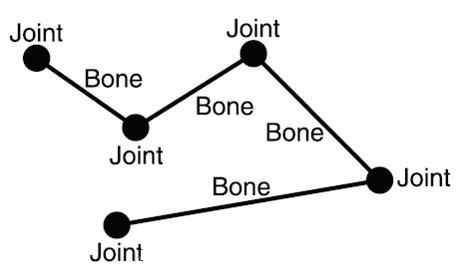
\includegraphics[width=.6\linewidth]{SkeletonTheory01}
					\caption{骨头、关节}
				\end{figure}
				
				当执行骨骼动画时,不必担心关节,或骨头之间的结合点。每个顶点实际上是附着(关联)到关节点的,而不是骨头。
			
			\paragraph{根关节}
				根关节是一个模型中的\textbf{终端关节}。任何其它关节都以自己的路径最终关联到根关节。
				
				任何对\textbf{根关节}的操作,如不论是平移或是旋转,都会影响到模型中的每个顶点。\textit{旋转或平移根关节将影响模型中其他所有的关节和项点。}
				
					\begin{figure}[H]
						\centering
						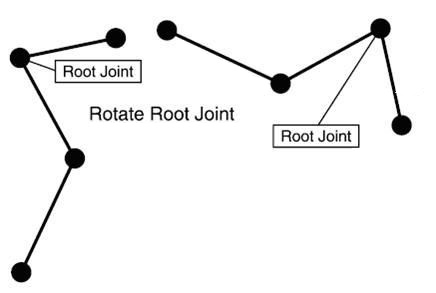
\includegraphics[width=.6\linewidth]{SkeletonTheory02}
						\caption{根关节}
					\end{figure}
				
				在每个模型里\textbf{只有一个根关节},它没有父关节。
				
				根关节通常是许多骨头连接的地方,而不是需要一个小动画的地方。\textit{例如包括中部和下后部,但没有明确要求根关节一定要在模型中的某个准确位置。}
			
			\paragraph{父关节和子关节}
				一个关节可以有父关节和子关节。
				
				\textbf{父关节的旋转和平移}\underline{会影响}计算\textit{当前关节的新位置}。
				
				\textit{再拿手臂的例子来说,肘关节是手掌的父关节。移动肘关节则影响手掌}。在简单的骨骼动画里,每个关节只有一个父关节,如果有的话。
			
				一个关节可以有许多子关节。\textit{任何你对父关节做的事都会渗透到子关节}。
				
					\begin{figure}[H]
						\centering
						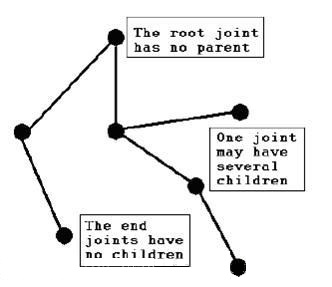
\includegraphics[width=.6\linewidth]{SkeletonTheory03}
						\caption{父子关节}
					\end{figure}				
				
			\paragraph{关键帧}
				关键帧 是一个模型位置的瞬时状态。
			
				不同于\textit{每个关键帧都包含其自身所有顶点的}\textbf{拷贝的方式},骨骼动画的关键帧或叫\textbf{骨骼帧(boneframe)}包含了\textit{旋转和平移的变换信息},一般平移是一个X,Y,Z值的形式,和三个分别包含了按X,Y,Z轴旋转的值。
				
				如常规顶点关键帧一样,\textbf{这些骨骼帧必须被插值来提供平滑的动画效果}。
				
				对弧形路径按两端点的直线方式而不是沿弧的路径方式进行插值就会产行“渗出”效果。解决这个问题的最好方法就是\textbf{采用四元数}来\textit{对旋转}进行插值。
				
			\paragraph{计算位置}
				如何更改它以使关节之间能正常运动。
				
				首先你要做的就是创建一个\textbf{变换矩阵},该矩阵用于每一个使用了不同旋转和平移关键帧数据的(关键帧)点。这个变换矩阵可以通过先\textbf{生成三个旋转矩阵}(译注:x,y,z三个方向的旋转矩阵)和\textbf{平移矩阵}。
				再将这三个矩阵相乘就会生成了最终的\textbf{变换矩阵}。
				
				你也可以使用matrix类的SetRotation和SetTranslation函数来避免你自己做矩阵乘法。这个生成的矩阵叫做\textbf{相对矩阵(relativematrix)}。
				
				下一步需要计算出一个\textbf{绝对矩阵(absolute matrix)}。绝对矩阵是\textit{关节的相对矩阵}\underline{乘上}它的\textit{父关节的绝对矩阵}得到的。绝对矩阵告诉你关节的绝对变换(译注:就是将关节的本地坐标变换为世界坐标)。这包括了自身的相对变换,除此之外,层次结构中所有在它之前的关节的变换都已计算完成。这允许其他关节的移动作为移动关节链上游关节的结果。细想一下,例如,当你移动肩膀时肘又是怎么移动的,这引出了一个问题:你如何计算最初的绝对矩阵?\textit{根关节是没有父关节的,因此,它的绝对矩阵就是它的相对矩阵}。
				
					\begin{figure}[H]
						\centering
						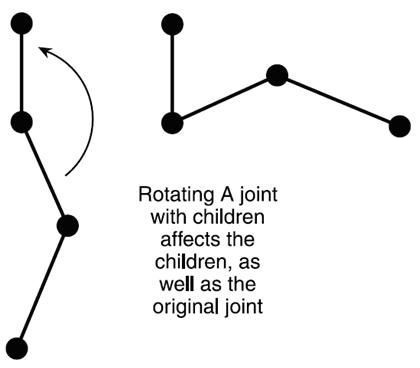
\includegraphics[width=.6\linewidth]{SkeletonTheory04}
						\caption{旋转一个关节并影响其子关节群}
					\end{figure}
					
				如上图所述:遍历各关节,会顾及其所有前面的变换。\textit{哪怕只有一个关节要移动,在它下面的关节也得跟着移动},这很像移动你的臀部,则你的膝和踝也得跟着移动一样。
				
				骨骼帧不会被累积,每帧保存了从起点起的特定关节的旋转和平移的信息。如果你不回退到原始顶点,那么当每次计算新顶点位置时,模型将会飘乎不定得运动。
			
			\paragraph{将网格附着到骨骼}
				当关节己能平滑运动的时候,也是该将网格附着到骨骼的时候。
				
				\textbf{网格(mesh)组成了模型的形状,它是由一组使模型具有立体感和细节的顶点和三角形组成,没有网格,基于骨骼运动的模型只是一个简单的骨架。每个网格的顶点存储了一个指向关节数组的索引,用于指示它被附着到某根骨头}。
					\begin{figure}[H]
						\centering
						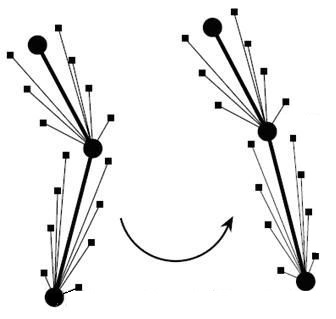
\includegraphics[width=.6\linewidth]{SkeletonTheory05}
						\caption{顶点附着于关节}
					\end{figure}
				
				每个模型包含了一个\textbf{纹理坐标的集合}和一个\textbf{三角形信息的集合}。仅因为\textbf{顶点的位置变更}并不意味着\textbf{三角形顶点索引}和\textbf{纹理坐标}也会变化。这意思是说,当第一次设置好它们之后就根本不需要再担心它们。
				
				法线则是另一回事了,因为多边形的朝向和顶点的位置更改了,因此法线也相应更改了。如果你正在使用面法线,那么你在每一帧将他们传给渲染器之前都需要重新计算。然而,如果你一开始就计算了顶点法线,那么你很幸运,顶点法线不必在变换后都完全重新计算,它们能利用和顶点相同的变换矩阵来进行变换。唯一不同的是,你不需要考虑平移。
				
				另一个需要考虑的问题是,顶点如何附着到多于一根的骨头。此时,每根骨头将被赋予一个权重,这个权重决定它影响关节点的比重。最终的变换是所有这些被附着的骨头的变换的加权平均。
	

	\section{骨骼动画UE4 基本概念}
			动画系统概念介绍:ref url:\url{https://zhuanlan.zhihu.com/p/62401630}
			
			创建人物角色动画蓝图:ref url:\url{https://blog.csdn.net/alzzw/article/details/104727955/}
			
		\subsection{概述}
			\begin{figure}[H]
				\centering
				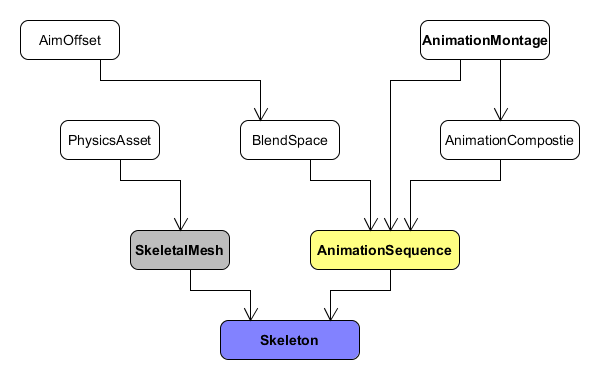
\includegraphics[width=.9\linewidth]{Anim_datas}
				\caption{UE4常见动画资源关系图}
			\end{figure}


			\begin{figure}[H]
				\centering
				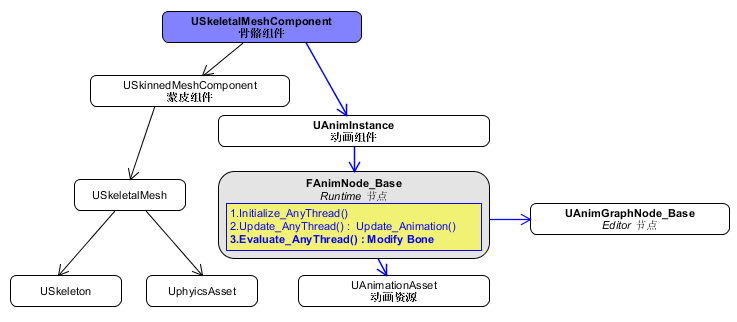
\includegraphics[width=.9\linewidth]{Anim_datas01}
				\caption{UE4骨骼动画资源关系图}
			\end{figure}		
		
			\paragraph{Skeleton 骨骼}
				是整个\textbf{动画系统的基础},其主要作用是记录了骨架以下信息:
				
				\begin{itemize}
					\item USkeleton : \verb|USkeleton|并不会直接使用自身的数据而是会生成一个\verb|FReferenceSkeleton|来提供给mesh来使用。
					\item 骨骼层级信息 :
					\item 参考姿势信息 :
					\item 曲线(Curve)信息
					\item 动画通知(Animation Notify)信息
					\item 插槽数据(插槽名称、所属骨骼、Transform等)
					\item 骨骼名称Index映射表、其他骨骼设置信息(位移重定向(Translation Retarget)设置,LOD设置等)
				\end{itemize}
			
			\paragraph{Skeletal Mesh 骨骼模型}
				骨骼模型是\textbf{在骨骼基础之上}的模型,通俗来说就是绑定骨骼后的网格体,也就是我们在游戏中能够看到的角色的\textbf{“肉身”}。
				\begin{itemize}
					\item USkeletalMesh: 链接Mesh和动画的桥梁
					\item 模型的顶、线、面信息
					\item 顶点的骨骼蒙皮权重
					\item 模型的材质信息
					\item 所属骨架
					\item Morph Target、Physics Asset、布料系统 等设置
				\end{itemize}
			
			
			\paragraph{Animation Sequence 动画序列}
				是用来记录骨骼运动状态的资源,也是让动画动起来的关键之一,其主要包含了一下信息:
				
				\begin{itemize}
					\item 动画\textbf{关键帧}信息
					\item 包含运动的骨骼信息
					\item \textbf{每帧骨骼的Transform信息}:包含了骨骼的旋转、位移和缩放
					\item 动画通知信息:记录了触发通知的类型和时间
					\item 动画曲线信息:记录了随时间轴变化的曲线信息
					\item 其他基础信息:包括了叠加动画设置、根骨骼位移设置等信息
				\end{itemize}
			
			\paragraph{BlendSpace 混合空间}
				
					\subparagraph{AimOffset}
								AimOffset\textit{ 是BlendSpace的一种特殊形式},区别在于其内部的所有采样点都是叠加动画。主要用在游戏过程中叠加角色瞄准和看的方向。
			
			\paragraph{动作融合}
			
			
			\paragraph{叠加动画}
			
			
			\paragraph{AnimationMontage}
				\verb|AnimationMontage|(简称Montage)是对\verb|Animation Sequence|等资源的扩充,可以方便的使用蓝图、代码控制动画资源的播放,并且可以方便的实现根骨骼动画和动画播放结束后的回调。
				
				要使用\verb|Montage|就需要将相应的动画拖入其中,在\verb|Montage|编辑器中可以对动画进行编辑、裁剪、拼接等操作(详情请见官方文档)。
				
				\verb|Montage|编辑器中有一个 \verb|Slot|(插槽)的东西,通俗的解释就是,插槽是对应在动画蓝图中播放\verb|Montage|的\textbf{播放点},同一个\verb|Montage|可以有多个不同的\verb|Slot|。另外Montage的使用上还有 \verb|Section| 等概念,具体使用方式在未来讲到动画系统搭建的时候会具体解释。
			
			
			
			\paragraph{动画节点}
				
				\subparagraph{分类}
					
					\begin{itemize}
						\item \verb|FAnimNode_Base|:{运行时的行为节点}
						\item \verb|UAnimGraphNode_Base| :{编辑器的图表节点},依赖FAnimNode 实际处理。
						\item \verb|FAnimNode_AssetPlayerBase|: 播放动画的节点父类,大部分工作都是对于\verb|UAnimSequence| 资源类型的更新
					\end{itemize}
					
					
				\subparagraph{核心函数}
				
					\begin{itemize}
						\item \verb|Initialize_AnyThread()|:当节点第一次运行时,会运行\verb|Initialize_AnyThread|。
						\item \verb|CacheBones_AnyThread()|:CacheBones用于刷新该节点所引用的骨骼索引。
						\item \verb|Update_AnyThread()|:更新
						\item \verb|Evaluate_AnyThread()|:调用以根据Update()中设置的权重计算局部空间\textbf{骨骼变换}。
						\item \verb|FPoseLink SourcePose()|;这是在节点上的pose连结点,会串联出来基本的运行逻辑。基本上每个animNode都会。
					\end{itemize}		
					
				
				\subparagraph{连接点}
					\begin{itemize}
						\item FPoseLink
						\item FPoseLinkBase
					\end{itemize}
					
						
						
			
			
			\paragraph{Animation Instance}
				这是所有逻辑的控制中心。
			
			
			
			\paragraph{Animation Blueprint}
			
			
			
			
		\subsection{角色动画:骨骼动画系统}
			
			\paragraph{大流程}
				大致如下:
				
				\begin{enumerate}
					\item \textbf{计算骨骼Pose}
						
						每一根骨骼可以看做一个点,而Pose就是所有骨骼Transform(位移+旋转+缩放)的集合,注意,一般来说,这个Pose 是\textit{基于骨架参考姿势}(Reference Pose)的\textbf{变换矩阵}。
					\item \textbf{蒙皮}
					
						将3D美术制作好的\textit{网格体的顶点按照骨骼Pose进行变化}。这里变换的依据是顶点的\textit{蒙皮权重}和\textit{参考姿势}的信息(一个顶点可能受到多个骨骼的影响)。
				\end{enumerate}
				
			\paragraph{更新流程}
				UE4里主要承担这两步职责的是\verb|Skeletal Mesh Component|。
				
				\verb|SkeletalMeshComponent| 继承自 \verb|SkinnedMeshComponent|。在\verb|SkeletalMeshComponent|创建时,会创建一个\verb|Animation Instance|,\textbf{这就是主要负责计算最终Pose的对象},而我们制作的 \verb|AnimationBlueprint| 也是基于 \verb|UAnimationInstance| 这个类的。
				
				在\verb|SkeletalMeshComponent| 进行 \verb|Tick()| 时,会调用 \verb|TickAnimation()| 方法,然后会调用 \verb|Animation Instance| 的 \verb|UpdateAnimation()| 方法,此方法会调用一遍所有动画蓝图中连接的节点的 \verb|Update_AnyThread()| 方法,用来\textbf{更新所有节点的状态}。
				
				然后后续 \textit{根据设置的不同} 会从 \verb|Tick()| 函数或者 Work线程中 调用 \verb|SkeletalMeshComponent| 的 \verb|RefreshBoneTransforms()| 方法,此方法进而会调用动画蓝图所有节点的 \verb|Evaluate_AnyThread()| 方法。
				
				\verb|Evaluate| 的含义就是指 \textit{根据特定的条件(从 Update() 时获得的参数)} 计算出 动画\textbf{所有骨骼的Transform信息},最后 \textbf{输出一个Pose 给到渲染线程} 并存在本地Component上。
				
				简化下的流程如下:
				\begin{itemize}
					\item \verb|Init()| 初始化
					\item \verb|Update()| 动画蓝图从游戏逻辑中收集状态变量并更新骨骼位置
					\item \verb|Evaluate()| 根据骨骼位置对动画进行解压和混合
					\item \verb|Complete()| 将运算后的顶点数据推送到渲染现场,更新物体位置和动画通知
				\end{itemize}
				
				
			\paragraph{AnimInstanceProxy}
				属于\textit{多线程优化动画系统}的核心对象。可以分担动画蓝图的更新工作,\textbf{将部分动画蓝图的任务分配到其他线程去做}。
			
			
			
		\subsection{IK}
		
		
		\subsection{其他}
		
		
				
	\section{流程}
	
	
	\section{深入}
	
	
	
\chapter{粒子系统}
							
\chapter{资源管理}

\chapter{Editor 扩展}
		
\chapter{跨平台发布apk}

\chapter{Profile}
	
\chapter{UE4 优化}

\chapter{调试技巧}
	
	
	
	
	
\end{document} 
 		    